If the mouse points to a graphical object, some key command has to be performed, for example to mute an audio clip, or modify the gain of a track. A key command is a single key press, a combination of key presses, or a key hold action in combination with a mouse movement. The following description shows how the different categories of key actions are notated and how they are performed.

\begin{description}
\item[Single Key Action \sact{K} -- Press and Release:]
This reads as: ``Press and Release a Key'', just like typing in a letter.
``K'' is the key to be used. (\emph{Note:} Even though capital letters are used to write down these actions, you should just press the ``K'' key and never use shift or caps lock, unless it is explicitly mentioned.) For example:
\begin{quotation}
   \sact{F}
\end{quotation}
means press and release the ``F'' key.

\item[Single Key Action \hact{K} -- Press and Hold:]
This reads as: ``Press and Hold the Key''. In a text editor you would get lots of kkkkkkkkkkk\dots.
Again, ``K'' is the letter associated with this action. For example:
\begin{quotation}
   \hact{D}
\end{quotation}
means press and hold the ``D'' key.

Hold keys in itself don't do anything. However if a ``hold key'' is active, and you move the mouse, an ``analogue'' action can be performed like moving an audio clip.

\item[Single Key Action \dact{K} -- Press and Release Twice:]
It reads as: ``Press and Release the key twice''. Like typing in one letter twice, rather fast, like a double click. For example:
\begin{quotation}
   \dact{G}
\end{quotation}
means press and release the ``G'' key twice.

\item[Double Key Action \sact{K K} -- Press and Release:]
This reads as: ``Press and Release 2 keys at once''. One of the more difficult actions. For example:
\begin{quotation}
   \sact{F G}
\end{quotation}
means press and release both the ``F'' and ``G'' key at the same time.

\item[Double Key Action \hact{K K} -- Press and Hold:]
It reads as: ``Press and hold 2 keys at once''. For example:
\begin{quotation}
   \hact{F G}
\end{quotation}
means press and hold at the same time both the ``F'' and ``G'' key.

The same idea applies as for the ``Single Key Action: Press and Hold'', however you have to press and hold 2 keys. This is a bit more difficult to do than with a Single Key Action, and is meant for more advanced usages/users.

\item[Double Key Action \dact{K K} -- Press and Release Twice:]
It reads as: ``Press and Release the 2 keys twice''. A difficult action to learn. Two keys have to be pressed and released at the same time, twice rather fast after each other! For example:
\begin{quotation}
   \dact{F G}
\end{quotation}
means press and release both the ``F'' and ``G'' key at the same time twice.

This key command isn't used much actually, due the fact that it's rather hard to perform. But this makes it an ideal candidate for destructive actions!
\end{description}

The cursor indicates which type of object is going to receive the key action by displaying a letter next to the cursor symbol. Hovering over a track it displays a T, over a clip a C, over a fade an F, and over a plugin a P (\FigB~\ref{fig_cursor}). If the key action is not known by the active object, the action is forwarded to the next object beneath the active object. For example in case of \hact{D} on a fade, the action is sent to the fade's audio clip.

From the menu ``Settings $\rightarrow$ Preferences\dots'', in the page ``Keyboard'' you can export or print the current keymap by pressing the buttons ``Export Keymap'' or ``Print Keymap''. This allows to have an up-to-date keymap always at your fingertips.

\begin{figure}[htb]
 \centering
 
\includegraphics[height=2\baselineskip]{../images/cursorFloatOverTrack.png}\qquad
 
\includegraphics[height=2\baselineskip]{../images/cursorFloatOverClip.png}\qquad
 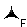
\includegraphics[height=2\baselineskip]{../images/cursorFloatOverFade.png}\qquad
 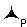
\includegraphics[height=2\baselineskip]{../images/cursorFloatOverPlugin.png}
 \caption{Depending on the type of object beneath the cursor, a letter is shown next to the arrow. From left to right: Track, Clip, Fade, Plugin.}
 \label{fig_cursor}
\end{figure}
